%***********************************************************
\subsection{MCMC Convergence}\label{sub:bc_mcmc_convergence}
%***********************************************************

% Introductory paragraph
The calibration schemes explained above were each run for a total of $2'000$ iterations using $1'000$ walkers. 
This results in a total of $2'000'000$ posterior samples.
These initial samples require further post-process\-ing to remove the initialization bias and the autocorrelation in the samples.
In the following, only the results from the calibration scheme with model bias term and considering all types of output (scheme \texttt{w/ Bias, All}) are discussed.
Though not shown, the results from other schemes are similar.

% Trace plots
Fig.~\ref{fig:ch5_plot_ens_trace_all_disc_centered} shows the trace plots for each of the $8$ model parameters in the calibration scheme \texttt{w/ Bias, All}.
To avoid over-plotting, the plot only shows the trajectories for the last $100$ iterations (out of $1'240$ post-burn-in iterations) and for $400$ walkers (out of $1'000$ walkers). 
As can be seen, the walkers traverse the model parameter space and spend more time during the iterations in the region where the values of the model parameters allows the simulator to best reproduce the experimental data (thus the region becomes darker in the plots).
Furthermore, it can be inferred that some parameters are more constrained by the data (e.g., \texttt{gridHT}) than the others (e.g., \texttt{tQuench}).

% Figure MCMC Ensemble Statistics
To check the convergence of an ensemble samplers, it is a common practice to investigate the running statistics of the ensemble (i.e., statistics over all walkers per iteration) instead of the individual walkers \cite{Foreman-Mackey2013,Akeret2013}.
The running average and standard deviation for each model parameter are shown in Fig.~\ref{fig:ch5_plot_ens_stat_mcmc}.
From the figure, it is clear that after some initial transient (i.e., the burn-in period), the running statistics converge for all parameters.
Note also that the number of iterations spent in the burn-in period for an ensemble sampler can be large (here up to $760$ iterations).
% Analyzing convergence
\begin{sidewaysfigure}
	\centering
	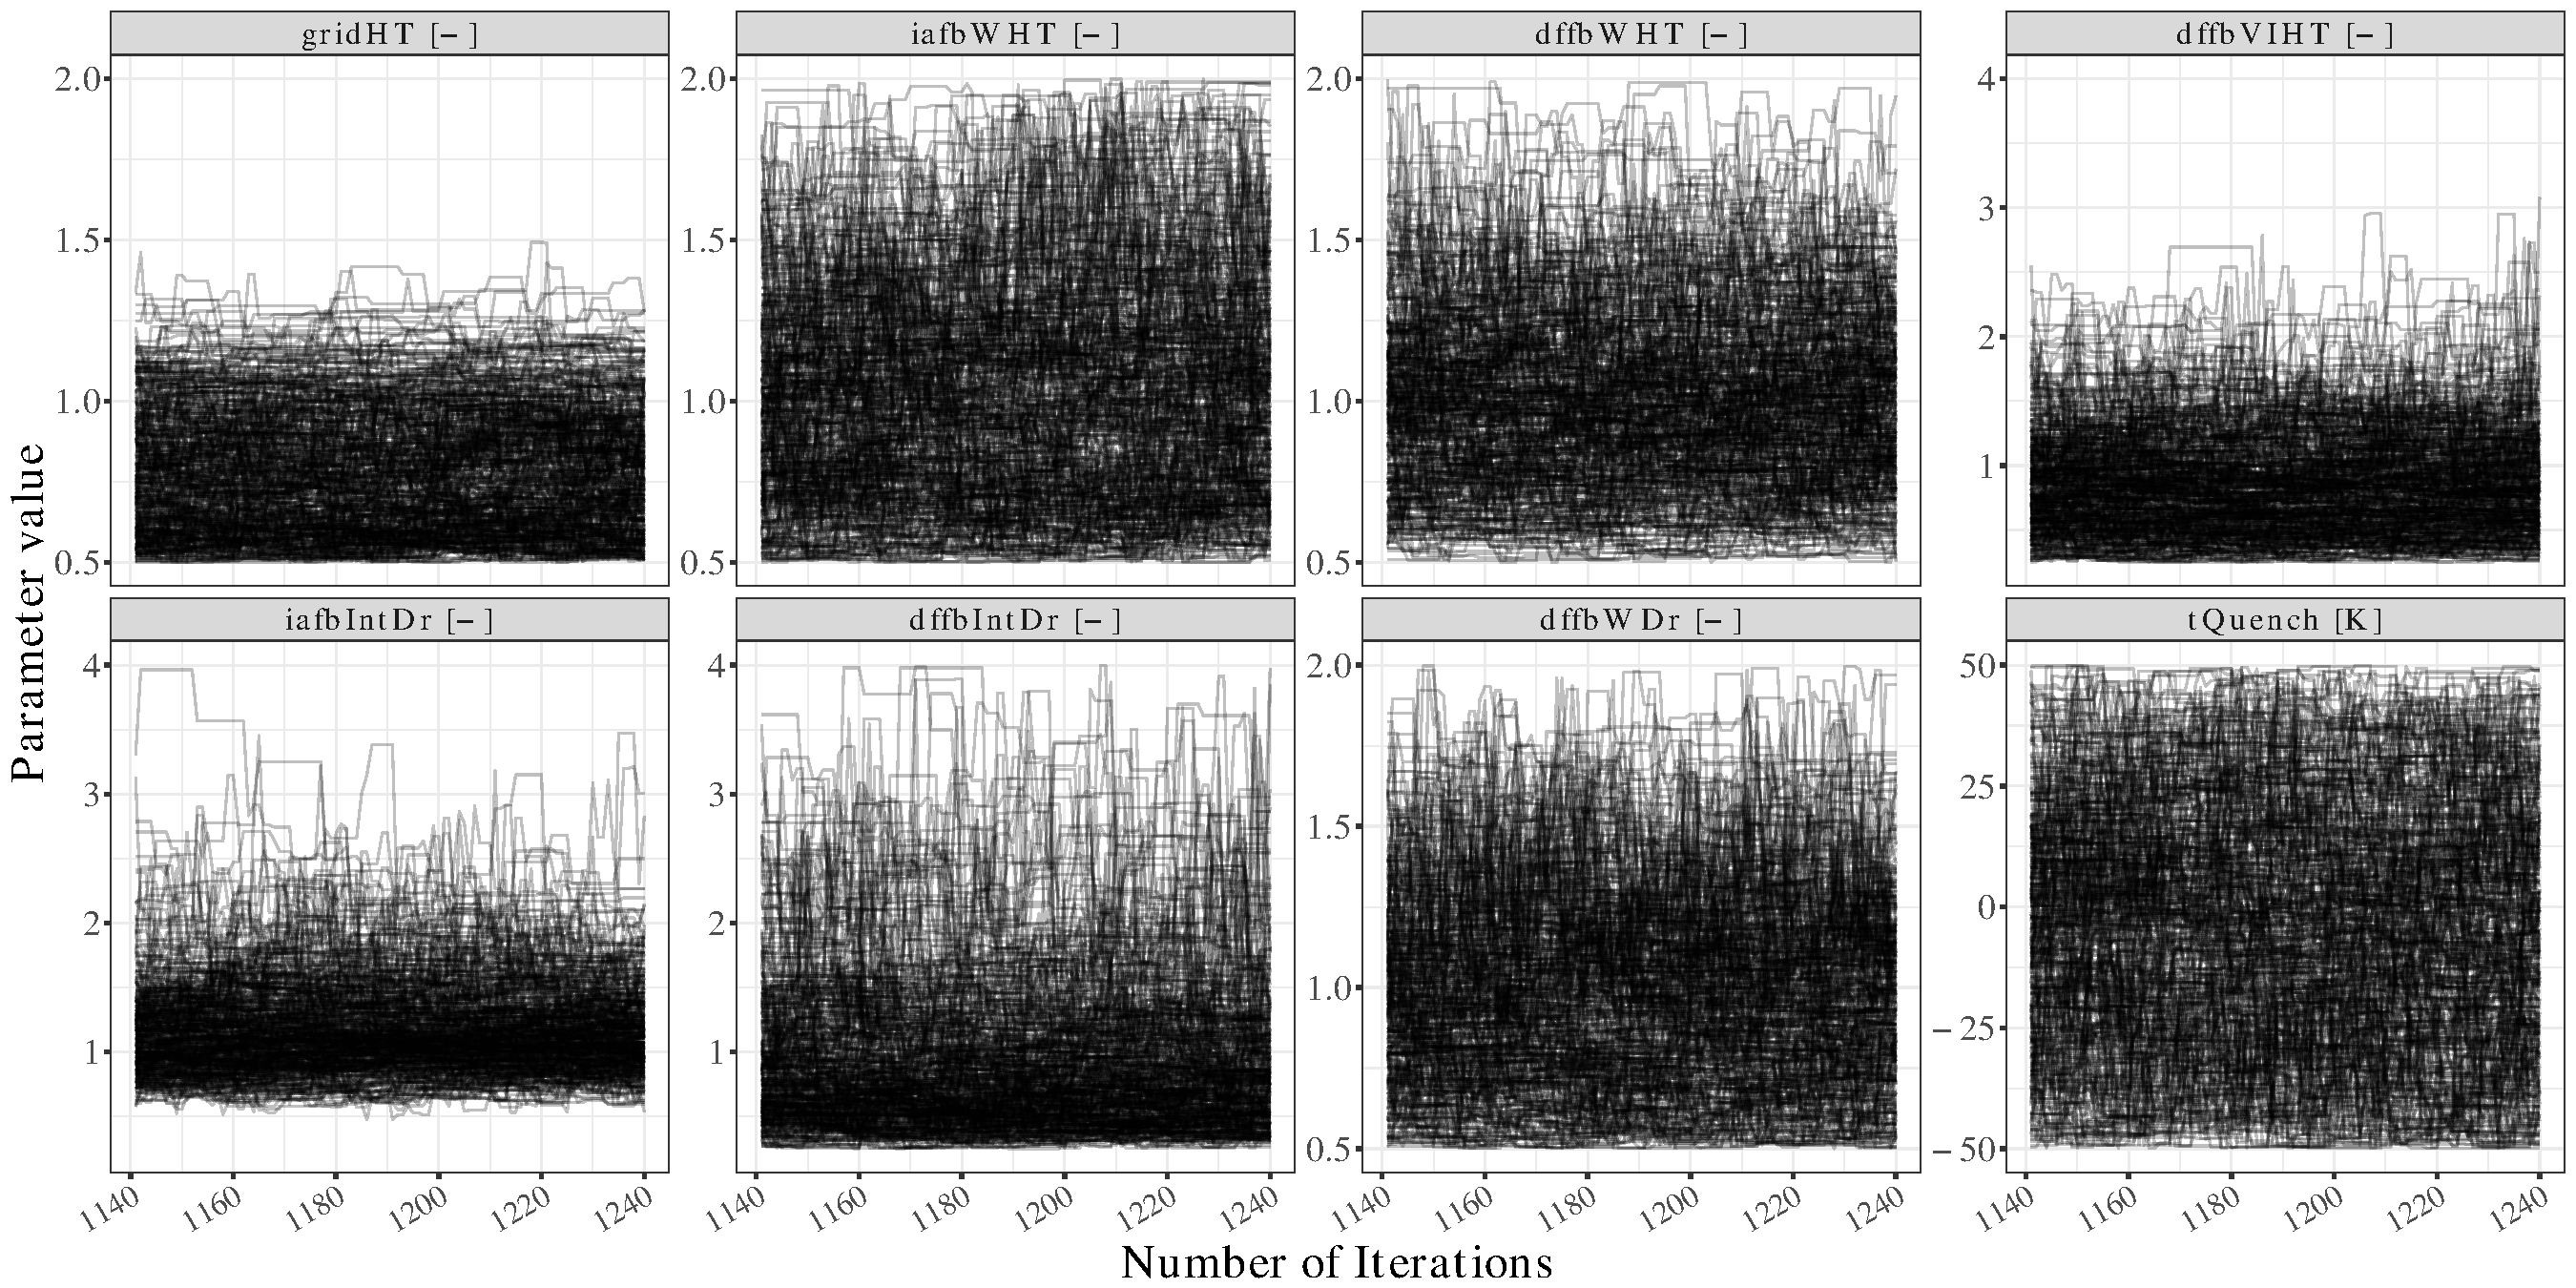
\includegraphics[width=0.90\textwidth]{../figures/chapter5/figures/plotEnsTraceDiscAllCentered}
		\captionof{figure}[Ensemble trace plots for each model parameter of calibration with model bias term.]{Ensemble trace plots for each model parameter of calibration with model bias term. Shown here are the last $100$ iterations (out of $1'240$ post-burn-in iterations) of $400$ walkers (out of $1'000$ walkers).}
	\label{fig:ch5_plot_ens_trace_all_disc_centered}
\end{sidewaysfigure}
\clearpage

\begin{figure}[!bth]
    \centering
    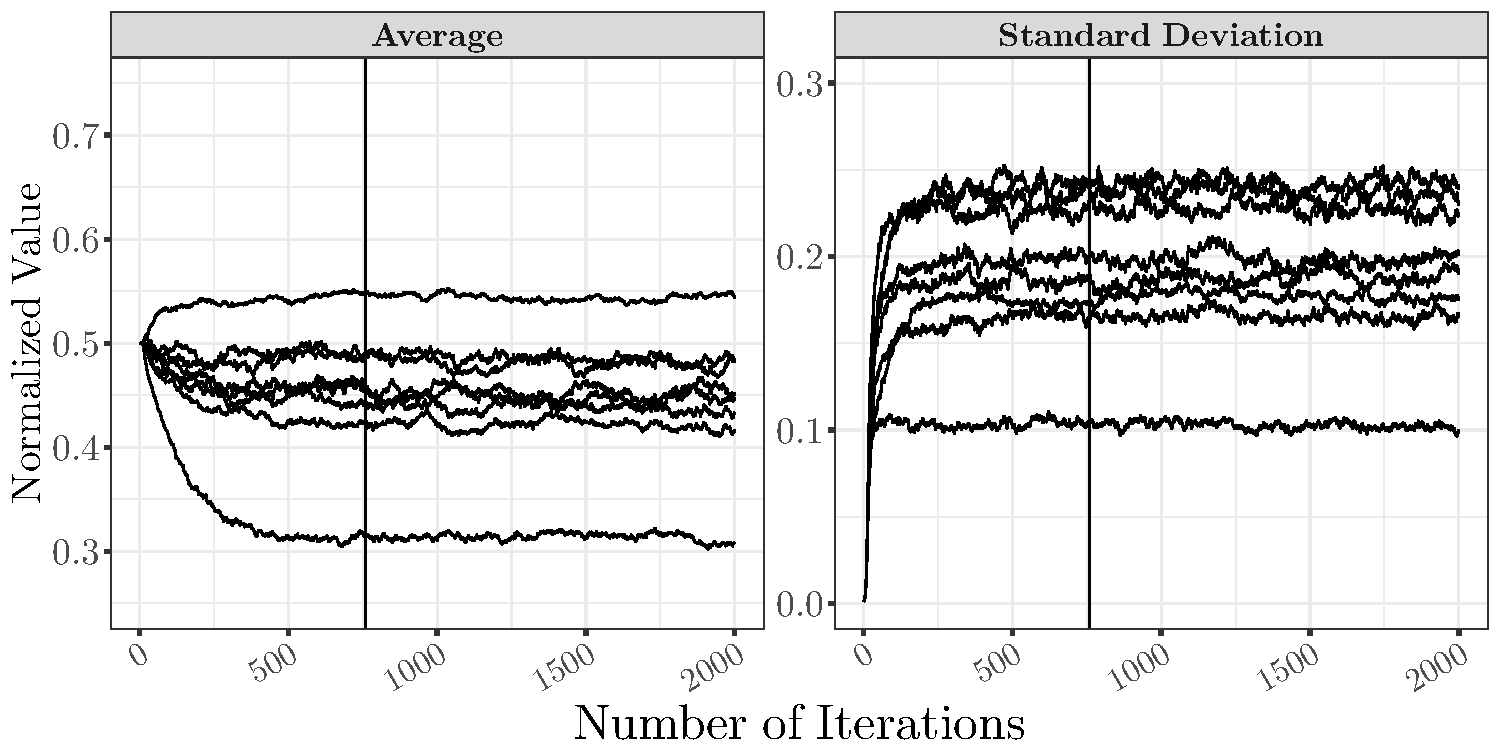
\includegraphics[width=1.0\textwidth]{../figures/chapter5/figures/plotEnsStatMCMC}
    \caption[Ensemble average and standard deviation as function of the number of iterations for calibration with model bias term.]{Ensemble average and standard deviation as function of the number of iterations for calibration with model bias term. Vertical lines indicate the iterations for burn-in (i.e., approximately $20$ times the autocorrelation time).}
    \label{fig:ch5_plot_ens_stat_mcmc}
\end{figure}

% Table of autocorrelation times, burn-in
Although the length of the burn-in period can be inferred directly from Fig.~\ref{fig:ch5_plot_ens_stat_mcmc}, a more rigorous criteria can be obtained via the autocorrelation time of the running statistics.
Table~\ref{tab:ch5_ens_stat_mcmc} summarizes the estimated autocorrelation time for the running statistics and for each model parameter.
The autocorrelation times of the average tend to be longer than the ones of the standard deviation. 
The longest autocorrelation time of all the parameters (shown in the table in bold) becomes the basis for determining the length of the burn-in period.
As recommended in \cite{Sokal1997} a multiple (in this case $20$) of the autocorrelation time is deemed enough to remove the initialization bias.
The obtained length of the burn-in period is shown as vertical lines in Fig.~\ref{fig:ch5_plot_ens_stat_mcmc} (at iteration $760$); those iterations are subsequently discarded.
\begin{table}[h]
	\myfloatalign
	\caption[Estimated autocorrelation times for the $8$ model parameters with respect to the ensemble running average and standard deviation, for the calibration scheme \texttt{w/ Bias, All}.]{Estimated autocorrelation times for the $8$ model parameters with respect to the ensemble running average and standard deviation, for the calibration scheme  \texttt{w/ Bias, All}. The bold term indicates the largest autocorrelation time used to determine the length of burn-in period.}
	\label{tab:ch5_ens_stat_mcmc}
	\begin{tabularx}{1.05\textwidth}{rlccccc} \toprule
		\multirow{2}{*}{No.}&\multirow{2}{*}{Parameter}		&\multicolumn{2}{c}{Average}	&\phantom{a}&\multicolumn{2}{c}{Standard Deviation}\\
																												\cmidrule{3-4}	                           \cmidrule{6-7}
      &												& $\tau_{\text{pre-burn-in}}$ 	& $\tau_{\text{post-burn-in}}$	&& $\tau_{\text{pre-burn-in}}$ & $\tau_{\text{post-burn-in}}$ \\ \midrule
		\footnotesize{1}	&	\footnotesize{\texttt{gridHT}	}			  & \footnotesize{$32.2$}  				& \footnotesize{$3.4$} 	      && \footnotesize{$15.1$}  		 & \footnotesize{$13.3$}\\
		\footnotesize{2}	&	\footnotesize{\texttt{iafbWHT}} 			& \footnotesize{$15.9$} 				& \footnotesize{$11.3$} 	    && \footnotesize{$12.2$}  		 & \footnotesize{$10.9$}\\
		\footnotesize{3}	&	\footnotesize{\texttt{dffbWHT}} 			& \footnotesize{$25.6$}  				& \footnotesize{$15.0$} 	    && \footnotesize{$13.4$}  		 & \footnotesize{$8.4$}\\
		\footnotesize{4}	&	\footnotesize{\texttt{dffVIHT}}			  & \footnotesize{$33.2$}  				& \footnotesize{$11.2$} 	    && \footnotesize{$14.1$}  		 & \footnotesize{$7.2$}\\
		\footnotesize{5}	&	\footnotesize{\texttt{iafbIntDr}} 		& \footnotesize{$28.6$}  				& \footnotesize{$\bm{19.4}$}  && \footnotesize{$10.7$}  		 & \footnotesize{$8.0$}\\
		\footnotesize{6}	&	\footnotesize{\texttt{dffbIntDr}} 		& \footnotesize{$\bm{37.8}$}  	& \footnotesize{$8.8$} 	      && \footnotesize{$14.3$}  		 & \footnotesize{$11.4$}\\
		\footnotesize{7}	&	\footnotesize{\texttt{dffbWDr}}			  & \footnotesize{$13.6$}  				& \footnotesize{$9.4$} 	      && \footnotesize{$25.1$}  		 & \footnotesize{$3.3$}\\
		\footnotesize{8}	&	\footnotesize{\texttt{tQuench}} 			& \footnotesize{$26.7$}  				& \footnotesize{$6.6$} 	      && \footnotesize{$14.1$}  		 & \footnotesize{$8.0$}\\
		\bottomrule
	\end{tabularx}
\end{table}

% Thinning
After such period, the autocorrelation time is re-estimated to assess if the sampler faces difficulty in sampling the posterior \gls[hyper=false]{pdf}.
A particularly long autocorrelation time, even after burn-in, gives an indication of a sampler that is trapped in a particular region of the parameter space \cite{Hou2012,Akeret2013} and thus requires longer iteration to have representative samples.
As can be seen in Table~\ref{tab:ch5_ens_stat_mcmc} ($\tau_{\text{post-burn-in}}$) the times are smaller after burn-in.

Additionally, the remaining samples are to be used for forward \gls[hyper=false]{uq}.
The \gls[hyper=false]{mc} simulation for forward \gls[hyper=false]{uq} requires independent (specifically, iid) samples.
To obtain a set of independent samples, the remaining samples are thinned on the basis of the re-estimated autocorrelation time (see Section~\ref{sub:bc_mcmc_thinning}.
The largest autocorrelation time of all parameters are used for thinning and $32'000$ independent posterior samples can be used for forward uncertainty propagation.
Though it results in a much smaller sample size, the associated statistical error relative to the standard deviation of the model parameter estimates are at most $0.6\%$ (Eq.~(\ref{eq:ch5_markov_chain_relative_error_ensemble})).
